% IEEE Journal of Biomedical and Health Informatics (J-BHI), regular submission.
% IEEE journal template (IEEEtran v1.8b, [journal] mode). Target decided 2026-11-26 (see ACTIVITY.md).
% Previous TCBB/compsoc skeleton (lineage-clone study) is in git history before this commit.
%
% Limits to confirm against the current J-BHI author guidelines (embs.org/jbhi) before drafting:
%   ~10 pages double-column (overlength charges beyond 8), abstract <= 250 words, index terms,
%   author bios/photos at acceptance.
%
% Numbers in the text come from generated/*.tex and tables/*.tex, written by scripts/ from
% committed results/ (scripts/paper_c2c2.py for registration II). Do not type results by hand.
% Registration-1 macros: TODO generator (aggregates in data/derived/models.json -> results/).
\documentclass[journal]{IEEEtran}

\usepackage{cite}
\usepackage{amsmath,amssymb}
\usepackage{graphicx}
\usepackage{booktabs}
\usepackage{url}
\usepackage[hidelinks]{hyperref}

\graphicspath{{figures/}}
\hyphenation{op-tical net-works semi-conduc-tor}

% AUTO-GENERATED by scripts/paper_c2c2.py from results/c2c2_*.json -- do not edit by hand.
\newcommand{\cctwoN}{47}
\newcommand{\cctwoAzeroOne}{44}
\newcommand{\cctwoBeta}{$-$0.57}
\newcommand{\cctwoSE}{0.26}
\newcommand{\cctwoP}{0.040}
\newcommand{\cctwoR}{$-$0.39}
\newcommand{\cctwoRlo}{$-$0.60}
\newcommand{\cctwoRhi}{$-$0.09}
\newcommand{\cctwoVisits}{527}
\newcommand{\cctwoBatchBeta}{$-$0.37}
\newcommand{\cctwoBatchP}{0.20}
\newcommand{\cctwoOldBeta}{$-$0.50}
\newcommand{\cctwoOldP}{0.073}
\newcommand{\cctwoAdjBeta}{$-$0.66}
\newcommand{\cctwoAdjP}{0.019}
\newcommand{\cctwoIdioP}{0.12}
\newcommand{\cctwoIdioN}{28}
\newcommand{\cctwoFiveP}{0.48}
\newcommand{\cctwoLooMin}{$-$0.75}
\newcommand{\cctwoLooMax}{$-$0.42}
\newcommand{\cctwoAfiveShare}{59}
\newcommand{\cctwoAfiveGenes}{78}
\newcommand{\cctwoHfourP}{0.66}
\newcommand{\cctwoSecN}{6}
\newcommand{\cctwoLeads}{895}
\newcommand{\cctwoLeadsQ}{1{,}024}
\newcommand{\cctwoTested}{28}
\newcommand{\cctwoConc}{0.96}
\newcommand{\cctwoPione}{0.79}
\newcommand{\cctwoNullConc}{0.68}
\newcommand{\cctwoNullPione}{0.21}
\newcommand{\cctwoExpressed}{689}
\newcommand{\cctwoOnArray}{46}
\newcommand{\cctwoArraySNPs}{249{,}458}
\newcommand{\cctwoBatchRtwoDtwo}{0.20}
\newcommand{\cctwoBatchPDtwo}{0.049}
\newcommand{\cctwoBatchRtwoSlope}{0.15}
\newcommand{\cctwoBatchPSlope}{0.15}
\newcommand{\cctwoRall}{$-$0.22}
\newcommand{\cctwoRwithin}{$-$0.17}
\newcommand{\cctwoRbetween}{$-$0.55}


\begin{document}

\title{Cell-to-Clinic: A Gated, Pre-Registered Test of Whether iPSC Dopaminergic-Neuron
Phenotypes Track Parkinson's Disease Progression}

\author{Victor~Ikenna~Kanu
        and~Dong-Seong~Kim%
\thanks{V.~I.~Kanu and D.-S.~Kim are with the Network Systems Lab, Kumoh National
Institute of Technology, Gumi, South Korea (e-mail: vkanu@kumoh.ac.kr).}}

\markboth{IEEE Journal of Biomedical and Health Informatics}%
{Kanu and Kim: Cell-to-Clinic}

\maketitle

\begin{abstract}
% <= 250 words. Written last, from the final results. Must state: data (FOUNDIN-PD / PPMI),
% gated pre-registered design (osf.io/s6w9c, osf.io/4pzxa), registration-1 null, registration-II
% primary (beta \cctwoBeta, p \cctwoP) and its batch attenuation, and the design implication.
\end{abstract}

\begin{IEEEkeywords}
Induced pluripotent stem cells, Parkinson's disease, single-cell RNA sequencing,
pre-registration, disease progression, dopaminergic neurons, equivalence testing.
\end{IEEEkeywords}

% ---------------------------------------------------------------------------
\section{Introduction}\label{sec:intro}
% Question: do donor-derived iPSC DA-neuron phenotypes track the donor's clinical progression?
% Why gates: reliability, cell identity and genetic validity must hold before any linkage.
% Contributions: (1) gated pre-registered framework; (2) registration 1 (all-cell, null);
% (3) DA-label refinement + G-eQTL positive control; (4) registration II with sensitivity and
% deviations reported in full. Cite EMBC 2027 companion (under review) for reliability/design.
% Refs: \cite{bressan2023foundin,marek2011ppmi,jerber2021population,nosek2018prereg}

% ---------------------------------------------------------------------------
\section{Data}\label{sec:data}
We use iPSC-derived dopaminergic-neuron data from FOUNDIN-PD~\cite{bressan2023foundin},
linked to clinical follow-up of the same donors in PPMI~\cite{marek2011ppmi}.

\subsection{FOUNDIN-PD iPSC differentiations}
% FOUNDIN-PD \cite{bressan2023foundin}: donor lines, day-65 scRNA-seq and bulk RNA, five
% differentiation batches, media change (E6). Counts only, via generated macros.

\subsection{PPMI clinical follow-up}
% PPMI \cite{marek2011ppmi}: OFF-state MDS-UPDRS III \cite{goetz2008mdsupdrs}, DaTscan putamen
% SBR, CSF alpha-syn SAA \cite{siderowf2023saa}, NSD-ISS \cite{simuni2024nsdiss}.
% Data download date; Project 150 access.

% ---------------------------------------------------------------------------
\section{Pre-Registered Framework and Gates}\label{sec:framework}
% Fig.~\ref{fig:gates}. Gates before linkage (A0-1 visits, A0-3 cells, A0-5 coherence, G-icc,
% G-cells, G-eQTL). Models: REML LMM, Satterthwaite df \cite{satterthwaite1946}; TOST at
% +/-0.40 with 90% CI \cite{lakens2017equivalence}; BH \cite{benjamini1995fdr}; classes
% supported / equivalent / inconclusive; partial r = t / sqrt(t^2 + df).

\begin{figure*}[!t]
\centering
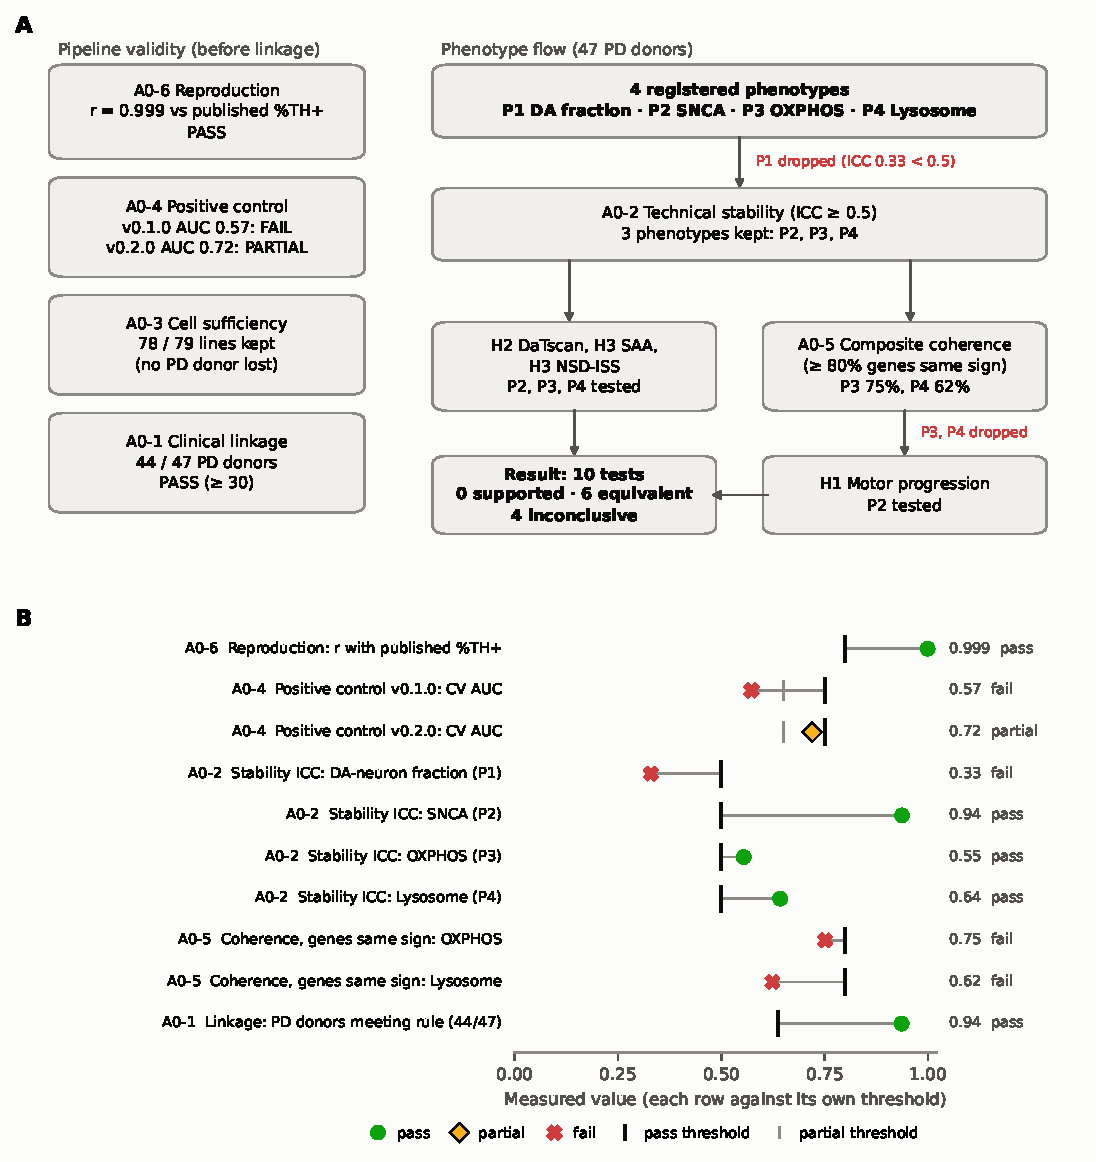
\includegraphics[width=0.72\textwidth]{fig1_gates.pdf}
\caption{Gated design. Each gate must pass before any phenotype is linked to clinical data.
% TODO caption from fig1 script.
}
\label{fig:gates}
\end{figure*}

% ---------------------------------------------------------------------------
\section{Registration 1: All-Cell Phenotypes}\label{sec:reg1}
% osf.io/s6w9c. Ten confirmatory tests; none supported (Fig.~\ref{fig:reg1}).
% Numbers via a registration-1 macro file (TODO generator).

\begin{figure*}[!t]
\centering
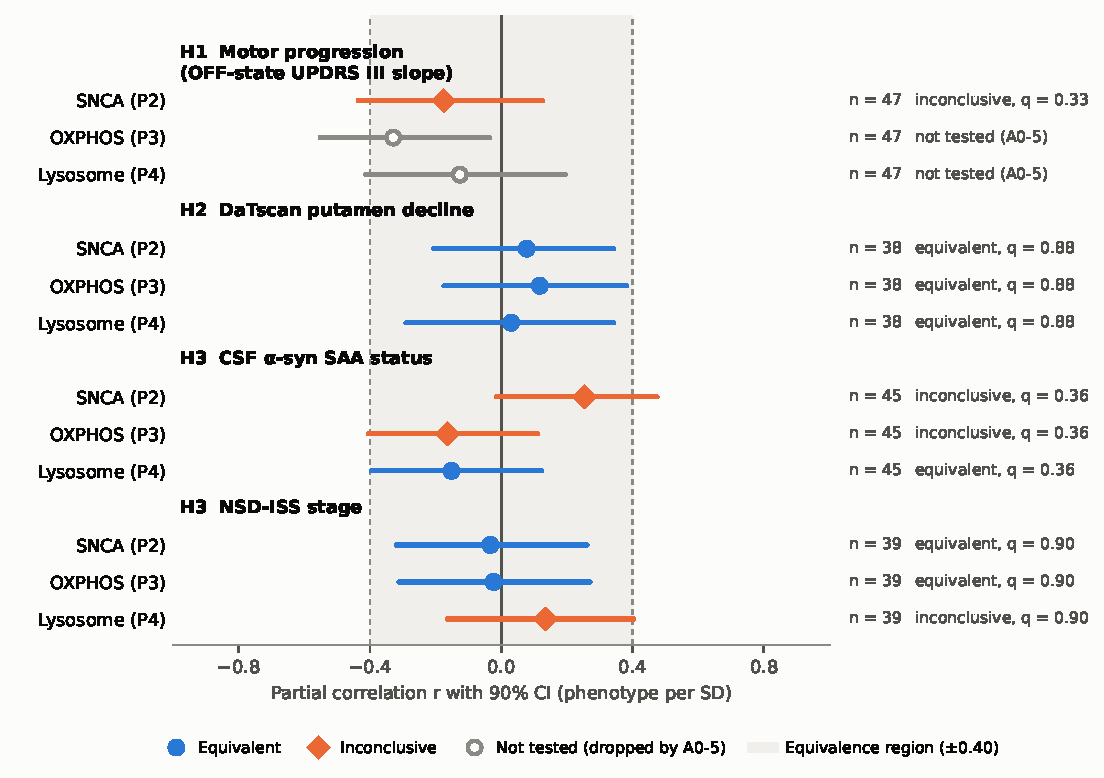
\includegraphics[width=0.9\textwidth]{fig3_forest.pdf}
\caption{Registration~1: partial correlation with 90\% CI for the confirmatory tests; shaded
region is the equivalence bound ($\pm 0.40$).}
\label{fig:reg1}
\end{figure*}

% ---------------------------------------------------------------------------
\section{DA-Neuron Phenotypes and Registration II Gates}\label{sec:reg2gates}
% DA-label refinement (new vs old label); phenotypes D1--D4; G-icc outcome (D1, D3 not tested).

% AUTO-GENERATED by scripts/paper_c2c2.py from results/c2c2_*.json -- do not edit by hand.
\paragraph{Genetic positive control (gate G-eQTL)}
Before any clinical linkage, we asked whether the new DA-neuron pseudobulks carry known DA-neuron genetic
regulation. Lead eQTLs were taken from day-52 untreated DA neurons of Jerber et al.\ (Supplementary Table~7;
one lead SNP per gene, gene-level empirical $p$ from 1{,}000 genotype permutations, BH FDR $<$ 5\%;
\cctwoLeads{} genes; \cctwoLeadsQ{} at Storey $q < 0.05$). Each lead was tested in the FOUNDIN DA pseudobulk
of the 79 donor lines by OLS of $\log_2$(CPM$+1$) on allele dosage with three genotype and five expression
principal components, after matching SNPs on GRCh37 position and alleles and dropping strand-ambiguous
SNPs. The gate passed if sign concordance with Jerber's $\beta$ was at least 0.70 and Storey's $\pi_1$
($\lambda = 0.5$) at least 0.30, both above the 95th percentile of 200 null sets pairing the same genes with
random SNPs on other chromosomes in the same MAF bin. Of the \cctwoLeads{} leads, \cctwoExpressed{} genes were
expressed (CPM $\ge$ 10) and only \cctwoOnArray{} lead SNPs were directly genotyped on the array
(\cctwoArraySNPs{} SNPs; no imputation or proxies were registered), leaving \cctwoTested{} testable pairs.
Concordance was \cctwoConc{} and $\pi_1$ \cctwoPione{} (null 95th percentiles \cctwoNullConc{} and
\cctwoNullPione{}); the gate passed, as it did for the old-label and all-cell pseudobulks. The gate therefore
shows that genetic regulation is present in the new label, not that the new label is more DA-specific.


% ---------------------------------------------------------------------------
\section{Registration II: Confirmatory Results}\label{sec:reg2}
% osf.io/4pzxa. Fig.~\ref{fig:reg2}.
Of the 47 PD donors, \cctwoAzeroOne{} met the visit rule (A0-1). For the primary test
(H1-DA), higher SNCA expression in DA neurons went with slower motor progression:
$\beta = \cctwoBeta$ UPDRS~III points per year per SD (SE \cctwoSE, $p = \cctwoP$; partial
$r = \cctwoR$, 90\% CI \cctwoRlo{} to \cctwoRhi; \cctwoVisits{} visits).
% Classification: supported. A0-5 for D4 failed (\cctwoAfiveShare\% of \cctwoAfiveGenes{}
% genes), so H1-D4 was dropped. Secondary family: \cctwoSecN{} tests, none supported.
% H4 bulk OXPHOS equivalent (p = \cctwoHfourP).

\subsection{Sensitivity analyses}
% Old label (p \cctwoOldP), composition-adjusted (p \cctwoAdjP), idiopathic only
% (n \cctwoIdioN, p \cctwoIdioP), batch covariate (beta \cctwoBatchBeta, p \cctwoBatchP),
% leave-one-out (\cctwoLooMin{} to \cctwoLooMax), first 5 years (p \cctwoFiveP).

\subsection{Exploratory, post hoc: batch structure}
% Label clearly. D2 by batch R^2 \cctwoBatchRtwoDtwo{} (p \cctwoBatchPDtwo); slope by batch
% R^2 \cctwoBatchRtwoSlope{} (p \cctwoBatchPSlope); r overall / within / between:
% \cctwoRall{} / \cctwoRwithin{} / \cctwoRbetween{} (n = 5).

\begin{figure*}[!t]
\centering
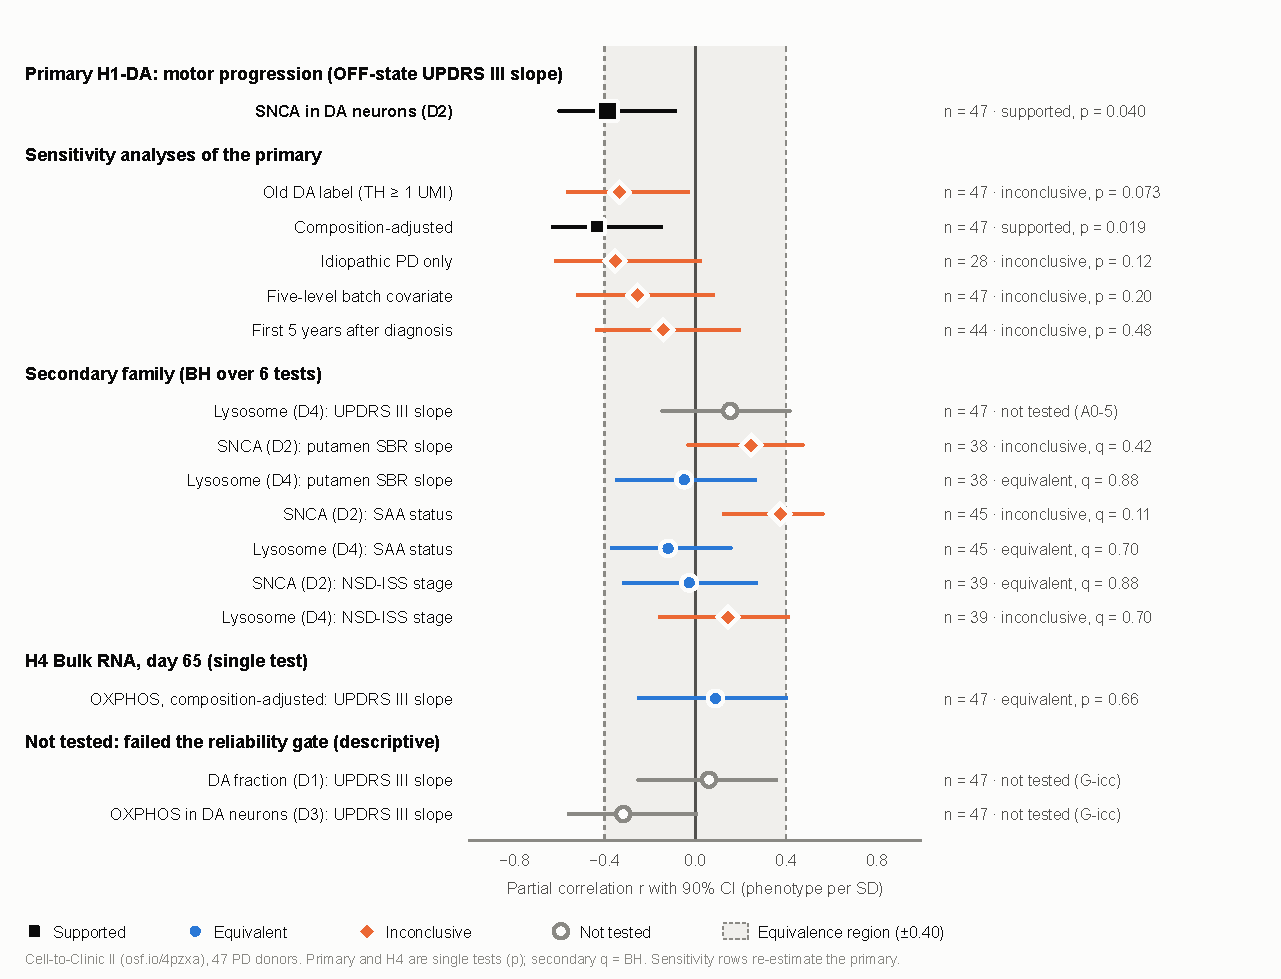
\includegraphics[width=0.85\textwidth]{fig5_c2c2_forest.pdf}
\caption{Registration~II: partial correlation with 90\% CI for the primary test, its
sensitivity analyses, the secondary family, H4 and the phenotypes not tested. Class is shown by
colour and marker shape; shaded region is the equivalence bound ($\pm 0.40$).}
\label{fig:reg2}
\end{figure*}

% ---------------------------------------------------------------------------
\section{Deviations from the Registrations}\label{sec:deviations}
% Table~\ref{tab:c2c2_deviations}. Registration-1 deviations: TODO.

% AUTO-GENERATED by scripts/paper_c2c2.py from results/c2c2_*.json -- do not edit by hand.
\begin{table*}[!t]
\centering
\caption{Deviations from the Cell-to-Clinic~II registration (osf.io/4pzxa) and post-hoc additions.}
\label{tab:c2c2_deviations}
\footnotesize
\begin{tabular}{p{2.6cm}p{4.2cm}p{4.6cm}p{5.4cm}}
\toprule
Item & Registered & Done & Reason / note \\
\midrule
G-eQTL lead source & Leads taken per gene from Jerber's all-SNP summary file (min-$p$ SNP, gene-level empirical $p$, BH). & Leads from Jerber et al.\ Suppl.\ Table~7 (context DA\_D52; same rule, BH FDR $<$ 5\%; 895 leads). & The released all-SNP files carry no gene-level $p$ (value $-1$ on every row). Decided before any FOUNDIN data was used; all 895 pairs found in the all-SNP file with identical $\beta$. \\
G-eQTL code version & Tagged before the run. & \texttt{g-eqtl-v1.0.0} failed on the real file (no leads); \texttt{g-eqtl-v1.1.0} used. & Failed version reported, not hidden. \\
Implementation readings & Not specified in the registered text. & H4 composition adjustment as for P3 in registration~1; A0-3 kept with G-cells; registration-1 SAA rule; sensitivity scope; D1/D3 descriptive. & Fixed in \texttt{models-da-v1.0.0} before linkage; accepted by the first author without independent review. \\
Post-hoc additions & -- & Batch check (\texttt{explore-II-v0.1.0}); eQTL attrition counts. & Labelled exploratory; specified and tagged before running. \\
\bottomrule
\end{tabular}
\end{table*}


% ---------------------------------------------------------------------------
\section{Discussion}\label{sec:discussion}
% Multiplicity across two registrations; batch attenuation (report both estimates);
% winner's curse for a narrowly met primary; direction vs registration-1 P2;
% design implications (cite EMBC companion); limitations (n = 47, single cohort, no
% external replication yet).

% ---------------------------------------------------------------------------
\section{Conclusion}\label{sec:conclusion}

% ---------------------------------------------------------------------------
\section*{Data and Code Availability}
% Registrations: osf.io/s6w9c, osf.io/4pzxa. Code and aggregate results: Zenodo
% 10.5281/zenodo.24156791, 10.5281/zenodo.24494010, 10.5281/zenodo.24526514.
% Participant-level data: PPMI and FOUNDIN-PD under their data use agreements.

\section*{Acknowledgment}
% PPMI acknowledgment (download date, RRID:SCR_006431, full funder list) and FOUNDIN-PD/MJFF
% wording, verbatim from the current PPMI publication policy.

\bibliographystyle{IEEEtran}
\bibliography{newref,c2c_refs}

\end{document}
